% REMEMBER TO SET LANGUAGE!
\documentclass[oneside, final, 11pt, english, twocolumn]{article}
\usepackage[utf8]{inputenc}
\usepackage[center]{titlesec}
% Standard stuff
\usepackage{relsize, amsmath, graphicx,varioref,verbatim,amsfonts, amssymb, setspace, makeidx,color, array}
% colors in text
\usepackage[usenames,dvipsnames,svgnames,table]{xcolor}
% Hyper refs
\usepackage[colorlinks=true, citecolor = blue]{hyperref}
\usepackage{lmodern}  
\usepackage{apacite}
\setcounter{secnumdepth}{0}
\usepackage{wrapfig}
\usepackage{subcaption}
\usepackage{float}
\usepackage{listings}
\setlength{\columnsep}{25pt} 
\usepackage{pythontex}
\usepackage{algpseudocode}
\usepackage[bottom]{footmisc}


\usepackage{stfloats}
\usepackage{breqn}



% Document formatting
% \setlength{\parindent}{0mm}
\setlength{\parskip}{1.5mm}
\setlength{\parindent}{24pt}

%Color scheme for listings
\usepackage{textcomp}
\definecolor{listinggray}{gray}{0.9}
\definecolor{lbcolor}{rgb}{0.9,0.9,0.9}
\usepackage{parskip}

%Listings configuration
\usepackage{listings}
\lstset{
	backgroundcolor=\color{lbcolor},
	tabsize=4,
	rulecolor=,
	language=python,
        basicstyle=\scriptsize,
        upquote=true,
        aboveskip={1.5\baselineskip},
        columns=fixed,
	numbers=left,
        showstringspaces=false,
        extendedchars=true,
        breaklines=true,
        prebreak = \raisebox{0ex}[0ex][0ex]{\ensuremath{\hookleftarrow}},
        frame=single,
        showtabs=false,
        showspaces=false,
        showstringspaces=false,
        identifierstyle=\ttfamily,
        keywordstyle=\color[rgb]{0,0,1},
        commentstyle=\color[rgb]{0.133,0.545,0.133},
        stringstyle=\color[rgb]{0.627,0.126,0.941}
        }
        
\newcounter{subproject}
\renewcommand{\thesubproject}{\alph{subproject}}
\newenvironment{subproj}{
\begin{description}
\item[\refstepcounter{subproject}(\thesubproject)]
}{\end{description}}


\usepackage{fancyhdr}
\fancyhf{} % sets both header and footer to nothing
\renewcommand{\headrulewidth}{0pt}
\fancyfoot[LE,RO]{\thepage}

\pagestyle{fancy}

%Lettering instead of numbering in different layers
%\renewcommand{\labelenumi}{\alph{enumi}}
%\renewcommand{\thesubsection}{\alph{subsection}}

\raggedbottom
\makeindex
\usepackage[totoc]{idxlayout}   % for index in the toc
\usepackage[nottoc]{tocbibind} 

%opening

\title{Project 1 FYS4150 - the 1D Poisson equation}% Force line breaks with \\

\author{Selma Beate Øvland}
\date{\today}

\begin{document}

\twocolumn[
  \begin{@twocolumnfalse}
    \maketitle
    \begin{abstract}
We solve the 1D Poisson equation using the LU decomposition method, and two algorithms that exploits the fact that we can solve the problem with a tridiagonal matrix. We compare the execution time of the algorithms, and see that by defining arrays for a tridiagonal matrix we can shorten the execution time and solve for much larger matrices than by using LU decomposition. We also calculate the relative error between our numerical solution and analytical solution, and see that for our algorithm the error decreases as n increases. 
    \end{abstract}
  \end{@twocolumnfalse}
]



\section{Introduction}

Many differential equations can be written as a linear second-order differential equation on the form

\begin{equation}
\frac{d^2}{dx^2} + k^2(x)y = f(x)
\end{equation}

where $f$ is the inhomogeneous term and $k^2$ is a real function. \\

In this project we will consider Poisson's equation

\begin{equation}
\Delta^2 \Phi = -4\pi \rho (\vec{r})
\end{equation}

where $\Phi$ is the electrostatic potential given by a localised charge distribution $\rho (\vec{r})$. We can simplify this equation by considering a spherically symmetric $\Phi$ and $\rho(\vec{r})$ to a one dimensional equation in r, given by

\begin{equation}
\frac{1}{r^2} \frac{d}{dr} (r^2 \frac{d\Phi}{dr}) = -4 \pi \rho(r)
\end{equation}

which via substitution ($ \Phi(r) = \phi(r)/r$) can be simplified further: 

\begin{equation}
\frac{d^2 \phi}{dr^2} = -4 \pi r \rho(r)
\end{equation}

We can define the inhomogeneous source term $f$ by $-4 \pi r \rho(r)$, and rewrite $\phi$ as $u$, and $r$ as $x$, so that we get

\begin{equation}
-u'' (x) = f(x)
\end{equation}

This is the one-dimensional Poisson's equation that we will solve in this project, by rewriting it as a set of linear equations. We have Dirichlet boundary conditions and a constraint on $x$:

\[x \in (0,1), \,\,  u(0) = u(1) = 0 \]

We also have a solution for the source term $f(x) = 100 e^{-10x}$, and an analytical solution to test our numerical calculations up against, given by 

\begin{equation}
v(x) = 1 - (1-e^{-10})x - e^{-10x}
\end{equation}

We will also calculate the relative error between our numerical and analytical solution:

\begin{equation}
\epsilon_i = log_{10}(\vert \frac{u_i - v_i}{v_i} \lvert )
\end{equation}


\section{Algorithms}

We will first define the discretized approximation to $u$ as $v_i$ with grid points $x_i =  ih$ in the interval from $x_0 = 0$ to $x_{n+1} = 1$. Step length is defined as $h = \frac{1}{(n+1)}$. Our boundary conditions are $u_0 = u_{n+1} = 0$. We can approximate the second derivate of $u$ by using Taylor expansion; 

\begin{equation}
- \frac{u_{i+1} + u_{i-1} - 2u_i}{h^2} = f_i
\label{eq:approx}
\end{equation}

where $i = 1,....,n$ and $f_i = f(x_i)$. When we want to rewrite the one-dimensional Poisson equation as a set of linear equations, we use the approximation from equation \eqref{eq:approx}, and end up with a set of equations. 

We define $\tilde{f_i} = h^2 f_i$ to simplify. 

We write out the terms in \eqref{eq:approx} from $i = 1$ to $i = n$ and we do not include the end points since these are given in the project description: 


\begin{align*}
i = 1; \, \, \, \, \, -u_2 - u_0 + 2u_1 = \tilde{f_1} \\
i = 2; \, \, \, \, \, -u_3 - u_1 + 2u_2 = \tilde{f_2} \\
i = 3; \, \, \, \, \, -u_4 - u_2 + 2u_3 = \tilde{f_3} \\
\vdots \\
i = n; \, \, \, \, \, -u_{n+1} - u_{n-1} + 2u_n = \tilde{f_n} \\
\end{align*}

From linear algebra we know that we can write the coefficients as a matrix

\[
    \mathbf{A} = \begin{bmatrix}
                           2& -1& 0 &\dots   & \dots &0 \\
                           -1 & 2 & -1 &0 &\dots &\vdots \\
                           0&-1 &2 & -1 & 0 & \vdots \\
                           \vdots & \vdots   & \vdots &\ddots   &\vdots & \vdots \\
                           0&\dots   &  \dots &-1 &2& -1 \\
                           0&\dots    &  \dots & 0  &-1 & 2 \\
                      \end{bmatrix},
\]

We also define two vectors

\[
\tilde{\mathbf{f}} = 
\left[ {\begin{array}{ccc}
\tilde{f}_1  \\
\tilde{f}_2  \\
\tilde{f}_3 \\
\vdots \\
\tilde{f}_n \\
\end{array} } \right]
\]

\[
\mathbf{u} = 
\left[ {\begin{array}{ccc}
u_1  \\
u_2  \\
u_3 \\
\vdots \\
u_n \\
\end{array} } \right]
\]

This translates the Taylor approximation in \eqref{eq:approx} to a matrix-vector product, where $\mathbf{u}$ is our unknown. 

\begin{equation}
\mathbf{A}\mathbf{u} = \tilde{\mathbf{f}}
\label{eq:linalg}
\end{equation}

As stated earlier $\tilde{f_i} = h^2 f_i$ , and the source term is $f(x) = 100 e^{-10x}$. 


\subsection{Gaussian Elimination - general tridiagonal matrix}

We want to make a general model that can work on any kind of tridiagonal matrix, so we define some vectors a, b and c to replace our coefficients in matrix $\mathbf{A}$. To simplify the walkthrough of our method, let's say we have a 4x4 matrix: 

\[
    \mathbf{A} = \begin{bmatrix}
                           b_1& c_1& 0 &0 \\
                           a_1 & b_2 & c_2 &0  \\
                           0&a_2 &b_3 & c_3 \\
                           0&0 & a_3 & b_4 \\
                      \end{bmatrix},
\]


And we want to solve the matrix-vector product $\mathbf{A}\mathbf{u} = \tilde{\mathbf{f}}$. 

\[
\left[
\begin{array}{cccc}

                           b_1& c_1& 0 &0 \\
                           a_1 & b_2 & c_2 &0  \\
                           0&a_2 &b_3 & c_3 \\
                           0&0 & a_3 & b_4 \\
\end{array}
\right] \cdot
\left[
    \begin{array}{c}
    u_1 \\
    u_2 \\
    u_3 \\
    u_4 \\
    \end{array}
    \right] = 
    \left[
    \begin{array}{c}
    \tilde{f_1} \\
    \tilde{f_2} \\
    \tilde{f_3} \\
    \tilde{f_4} \\ 
    \end{array}
\right] 
\]

To use Gaussian elimination (forward and backward substitution), we follow the steps from \cite[s. 170-173]{stat}we use the following matrix with 4 rows and columns

\[
    \begin{bmatrix}
                           b_1& c_1& 0 &0 & \tilde{f_1}\\
                           a_1 & b_2 & c_2 &0 & \tilde{f_2} \\
                           0&a_2 &b_3 & c_3 & \tilde{f_3}\\
                           0&0 & a_3 & b_4 & \tilde{f_4}\\
                      \end{bmatrix}
\]

Our first goal (with the forward substitution) is to transform all elements under the diagonal (lower left) to zeros. To achieve this we must multiply the element $b_1$ with $a_1/b_1$, which will replace the element $b_1$ with $a_1$.  We get a new temporary row 1: 

\[
\mathbf{row 1^*} = 
\left[ {\begin{array}{ccc}
a_1  \, \, \, \, \, 
c_1a_1 /b_1 \, \, \, \, \, 
0 \, \, \, \, \, 
0 \, \, \, \, \, 
\tilde{f_1} a_1/b_1 
\end{array} } \right]
\]



Then we can subtract this new row 1 from row 2 (but we will not actually change row 1 in our matrix), which gives us

\[
    \begin{bmatrix}
                           b_1& c_1 & 0 &0 & \tilde{f_1}\\
                           0 & b_2 - c_1 a_1 / b_1 & c_2 &0 & \tilde{f_2} - \tilde{f_1} a_1 /b_1\\
                           0&a_2 &b_3 & c_3 & \tilde{f_3}\\
                           0&0 & a_3 & b_4 & \tilde{f_4}\\
                      \end{bmatrix}
\]

We do a little substitution of variables; $b^*_2 = b_2 - c_1 a_1/b_1$, $f^*_2 = \tilde{f_2} - \tilde{f_1} a_1 /b_1$. 

\[
    \begin{bmatrix}
                           b_1& c_1 & 0 &0 & \tilde{f_1}\\
                           0 & b^*_2 & c_2 &0 & f^*_2\\
                           0&a_2 &b_3 & c_3 & \tilde{f_3}\\
                           0&0 & a_3 & b_4 & \tilde{f_4}\\
                      \end{bmatrix}
\]

Now we want to remove the second element, $a_2$,  on row 3. To do this we multiply row 2 with $a_2/b_2^*$; 

\[
\mathbf{row 2^*} = 
\left[ {\begin{array}{ccc}
0  \, \, \, \, \, 
a_2 \, \, \, \, \, 
c_2 a_2 /b_2^* \, \, \, \, \, 
0 \, \, \, \, \, 
f_2^* a_2/b_2^*\\
\end{array} } \right]
\]

And then subtract row 2* from row 3 to get: 

\[
    \begin{bmatrix}
                           b_1& c_1 & 0 &0 & \tilde{f_1}\\
                           0 & b^*_2 & c_2 &0 & f^*_2\\
                           0&0 &b_3 - c_2 a_2 /b_2^*& c_3 & \tilde{f_3} - f_2^* a_2/b_2^*\\
                           0&0 & a_3 & b_4 & \tilde{f_4}\\
                      \end{bmatrix}
\]

Again, we do a substitution of variables; $b^*_3 = b_3 - c_2 a_2/b_2^*$, $f^*_3 = \tilde{f_3} - f_2^* a_2 /b_2^*$. 

\[
    \begin{bmatrix}
                           b_1& c_1 & 0 &0 & \tilde{f_1}\\
                           0 & b^*_2 & c_2 &0 & f^*_2\\
                           0&0 &b_3^* & c_3 & f_3^*\\
                           0&0 & a_3 & b_4 & \tilde{f_4}\\
                      \end{bmatrix}
\]


For the fourth row, and third element; $a_3$, we want to multiply row 3 with $a_3/b_3^*$ and then subtract this row 3* from row 4. Following the same steps as above, we end up with the matrix

\[
    \begin{bmatrix}
                           b_1& c_1 & 0 &0 & \tilde{f_1}\\
                           0 & b^*_2 & c_2 &0 & f^*_2\\
                           0&0 &b_3^* & c_3 & f_3^*\\
                           0&0 & 0 & b_4^* & f_4^*\\
                      \end{bmatrix}
\]

where $b_4^* = b_4 - c_3 a_3/b_3^*$ and $f^*_4 = \tilde{f_4} - f_3^* a_3 /b_3^*$. 

We can from these steps see a pattern and derive two general algorithms for $b_i^*$ and $f^*_i$: 


\begin{equation}
b_i^* = b_i - c_{i-1}a_{i-1}/b_{i-1}^*
\end{equation}

\begin{equation}
f^*_i = \tilde{f_i} - f_{i-1}^* a_{i-1} /b_{i-1}^*
\end{equation}

These two algorithms removes all elements under the diagonal, and we are left with just two elements on the fourth row which makes it easy to achieve our next goal: turn the fourth element of row 4 into a 1. We just divide the entire row 4 by $b_4^*$ which turns the row into

\[
\mathbf{row \, 4} = 
\left[ {\begin{array}{ccc}
0  \, \, \, \, \, 
0 \, \, \, \, \, 
0\, \, \, \, \, 
1\, \, \, \, \, 
f_4^*/b_4^* \\
\end{array} } \right]
\]

This means we have a solution for the element $u_4 = f_4^*/b_4^*$, and with the 1 on the diagonal we can continue with the backward substitution and turn the upper triangular into zeros, from the bottom to the top. 

\[
    \begin{bmatrix}
                           b_1& c_1 & 0 &0 & \tilde{f_1}\\
                           0 & b^*_2 & c_2 &0 & f^*_2\\
                           0&0 &b_3^* & c_3 & f_3^*\\
                           0&0 & 0 & 1 & u_4\\
                      \end{bmatrix}
\]

With the above matrix, we multiply row 4 with $c_3$ so we get the following temporary row 

\[
\mathbf{row \, 4*} = 
\left[ {\begin{array}{ccc}
0  \, \, \, \, \, 
0 \, \, \, \, \, 
0\, \, \, \, \, 
c_3\, \, \, \, \, 
c_3 u_4 \\
\end{array} } \right]
\]

And then we subtract row 4* from row 3, and we also divide the whole row by $b_3^*$ and get the matrix

\[
    \begin{bmatrix}
                           b_1& c_1 & 0 &0 & \tilde{f_1}\\
                           0 & b^*_2 & c_2 &0 & f^*_2\\
                           0&0 &1 & 0 & (f_3^* - c_3 u_4)/b_3^*\\
                           0&0 & 0 & 1 & u_4\\
                      \end{bmatrix}
\]

where $u_3 = (f_3^* - c_3 u_4)/b_3^*$

For the next row we use the same logic, we multiply row 3 with $c_2$ and subtract this from row 2, then divide by $b_2^*$:

 \[
    \begin{bmatrix}
                           b_1& c_1 & 0 &0 & \tilde{f_1}\\
                           0 & 1 & 0 &0 & (f^*_2 - c_2u_3)/b_2^*\\
                           0&0 &1 & 0 & u_3\\
                           0&0 & 0 & 1 & u_4\\
                      \end{bmatrix}
\]

where we insert $u_2 = (f_2^* - c_2 u_3)/b_2^*$. 

We can do the same for the last (first) row, and again we see a pattern from where we can derive a general algorithm for $u_i$: 

\begin{equation}
u_i =  (f_i^* - c_i u_{i+1})/b_i^*
\end{equation} 

where i = n-1, ..., 1. 

So from gaussian elimination we have derived three algorithms, and our code needs to look something like this (pseudo code, python index): 

\begin{algorithmic}[H]
\State
\For {i in range 1, 2, ..., n}
	\State $ab = a_{i-1}/b^*_{i-1}$;
	\State $b^*_i = b_i - c_{i-1}* ab$
	\State $f^*_i = \tilde{f}_i - f^*_{i-1}* ab$;
\EndFor
\State
\State $u_{n-1} = f^*_{n-1}/b^*_{n-1}$;
\State
\For {i in range n-2, ..., 0}
	\State $u_i = (f^*_i - c_i*u_{i+1})/ b^*_i$;
\EndFor
\State
\end{algorithmic}


We can see from our pseudo code that the first loop uses 5 FLOPs and the second loop uses 3 FLOPs, making it a total of 8 FLOPs. Because we made a variable $ab$ we reduced the amount of FLOPs by one. Our total amount of FLOPs for this algorithm is therefore 5n -1 for the forward substitution, and 3n-1 for the backward substitution, but when n is large we can neglect the constant terms, so our total amount of FLOPs are 8n. 

\subsection{Special case - identical elements}

We are lucky since all the elements on the diagonal are identical, as well as all the elements under and above the diagonal (but different from each other). We can then simplify our code a little bit, as a, b and c are no longer arrays, but a constant. We insert a = c = -1 and b = 2 in our algorithms from the previous section and get: 

 
\begin{equation}
b_i^* = 2 - 1/b_{i-1}^*
\label{eq:btild}
\end{equation}

\begin{equation}
f^*_i = \tilde{f_i} + f_{i-1}^* / b_{i-1}^*
\end{equation}


\begin{equation}
u_i =  (f_i^* + u_{i+1})/b_i^*
\end{equation} 

If we look a little closer at \eqref{eq:btild}, we can see that there is an even simpler way of solving this algorithm. We know that $b_1^* = b_1 =  2$, and by solving for a few steps we can see a pattern:

\[b_i^* = 2 - \frac{1}{b_{i-1}^*} \]
\[b_2 = 2 - \frac{1}{2} = \frac{3}{2}\]
\[b_3 = 2 - \frac{1}{\frac{3}{2}} = \frac{4}{3}\]
\[b_4 = 2 - \frac{1}{\frac{4}{3}} = \frac{5}{4}\]
\[b_5 = 2 - \frac{1}{\frac{5}{4}} = \frac{6}{5}\]

Computing the results for a few steps forward, shows us a pattern in the values we get for $b^*$ and we can calculate these outside the loop we have previously computed $b^*$ in. We see from the above steps that $b^*$ can actually be computed the following way

\begin{equation}
d_i = \frac{i +1}{i}
\end{equation}

This new variable which we have called $d_i$, can now be calculated independently outside our forward and backward substitution loops. Our algorithm for the special case where the elements on the diagonal are identical, and the elements on the lower and upper diagonal are identical becomes; 


\begin{algorithmic}[H]
\State
\For {i in range 1, 2, ..., n}
	\State $f^*_i = \tilde{f}_i + f^*_{i-1}/d_{i-1}$;
\EndFor
\State
\State $u_{n-1} = f^*_{n-1}/d_{n-1}$;
\State
\For {i in range n-2, ..., 0}
	\State $u_i = (f^*_i + u_{i+1})/ d_i$;
\EndFor
\State
\end{algorithmic}

This reduces the amount of FLOPs for our algorithm. Here we have 2 FLOPs in the first loop, and 2 FLOPs in the second loop, making our total amount of FLOPs 4n, which is a drastic improvement from our general case, and means our program should run faster. 

\subsection{LU decomposition}

Another way of solving the set of equations from \ref{eq:approx} is to use LU decomposition. We will then rewrite our matrix $\mathbf{A}$ as a product of two matrices L and U where L consists of elements below the diagonal, and the value 1 on the diagonal, and U consists of elements only above and on the diagonal. We can use built in functions in python (or other programming languages) to get these matrices. \\

By following the steps in \cite[s.177-178]{stat}, when our system of linear equations is written on the form; $\mathbf{A}\mathbf{u} = \tilde{\mathbf{f}}$, we can use LU decomposition on $\mathbf{A}$ and get  

\begin{equation}
\mathbf{A}\mathbf{u} = \mathbf{LU} \mathbf{u} = \tilde{\mathbf{f}}
\label{eq:LU}
\end{equation}

We can calculate \eqref{eq:LU} in two steps

\begin{equation}
\mathbf{L}\mathbf{y} =\tilde{\mathbf{f}}; \;\; \; \; \; \; \; \mathbf{U}\mathbf{u} = \mathbf{y}; 
\end{equation}

From page 178 in \cite{stat} we see an example of a four dimensional matrix written out as a set of linear equations, using the above explained method: 


\begin{align*}
y_1 = \tilde{f}_1 \\
L_{2,1}y_1 + y_2 = \tilde{f}_2 \\
L_{3,1} y_1 + L_{3,2}y_2 + y_3 = \tilde{f}_3\\
L_{4,1}y_1 + L_{4,2} y_2 + L_{4,3}y_3 + y_4 = \tilde{f}_4 \\
 \\
\end{align*}

In our matrix $\mathbf{A}$ we only have elements on the diagonal, and the diagonal under and above it. So most elements in $\mathbf{A}$, $\mathbf{L}$ and $\mathbf{U}$ are equal to 0. That means we can eliminate some elements in the set of linear equations above, so it looks like this instead: 

\begin{align*}
y_1 = \tilde{f}_1 \\
L_{2,1}y_1 + y_2 = \tilde{f}_2 \\
L_{3,2}y_2 + y_3 = \tilde{f}_3\\
L_{4,3}y_3 + y_4 = \tilde{f}_4 \\
 \\
\end{align*}

We see a pattern here and can make a general algorithm: 

\begin{equation}
y_i = \tilde{f}_i - y_{i-1} L_{i,i-1}
\end{equation}

We look at the same equations for $\mathbf{U}\mathbf{u} = \mathbf{y}$ on page 178 from \cite{stat}, and we see that we can derive an algorithm for $\mathbf{u}$ here as well; 

\begin{equation}
u_i = y_i -  U_{i,i+1} u_{i+1} / U_{i,i}
\end{equation}

From looking at the set of linear equations we can also see that we need to do a forward substitution on $y_i$ and a backward substitution on $u_i$. Our code will look something like this: 


\begin{algorithmic}[H]
\State
\For {i in range 1, 2, ..., n}
	\State $y_i = \tilde{f}_i - y_{i-1} L_{i,i-1}$;
\EndFor
\State
\State $u_{n-1} = y_{n-1}$;
\State
\For {i in range n-2, ..., 0}
	\State $u_i = y_i -  U_{i,i+1} u_{i+1} / U_{i,i}$;
\EndFor
\State
\end{algorithmic}

From the lectures by Morten Hjorth-Jensen (on the 27th of August, 2020) we know that a LU decomposition requires $O(n^3)$ FLOPs. We will time the programs for different n, to see if there is a difference in execution time, and if there are any limits to how large n the programs can handle. 


\section{Results}

We have calculated the solution for our problem using the three different algorithms we found in the previous section. We get the same results for the solution $\mathbf{u}$ for all of them, but there is a big difference in execution time for all three methods, shown in table \ref{tab:time}. 

\begin{figure}[H]
\centering
    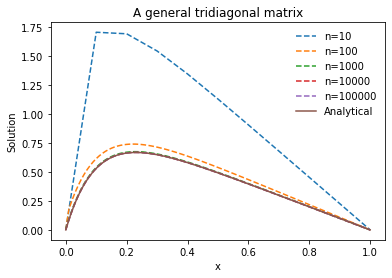
\includegraphics[width=0.8\columnwidth]{sol_general.png}
\caption{Our algorithm for a general tridiagonal matrix compared to the analytical solution. We can see that they are well matched for n=100 and higher. }
\label{fig:method1}
\end{figure}

\begin{figure}[H]
\centering
    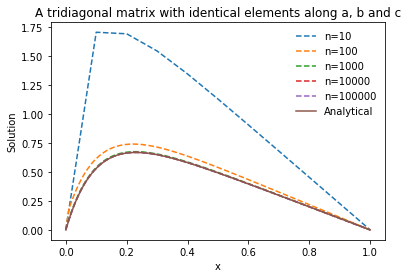
\includegraphics[width=0.8\columnwidth]{sol1.png}
\caption{Our algorithm used on a tridiagonal matrix where the elements along the diagonal a, b and c are known and identical within the array. For n=$10e2$ and higher we get very good results, where the solution matches the analytic solution very well. For some reason the results are not as good for n=10. Otherwise the results look identical to our algorithm for a general tridiagonal matrix (as it should). }
\label{fig:method2}
\end{figure}

From figure \ref{fig:method1} and \ref{fig:method2} it looks as if we get the same results for the two algorithms we derived by using Gaussian elimination. However, we do get a weird result for n = 10. I'm not sure why this happens, but the results are pretty close when n = 100 and higher. I removed the n = 10 results to show how close the results for hogher n were to the analytical solution in figure \ref{fig:bign}. 

\begin{figure}[H]
\centering
    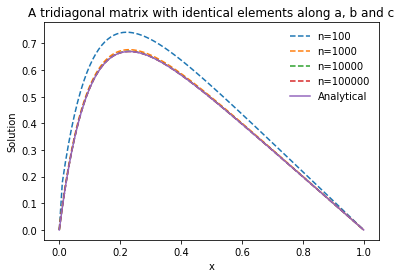
\includegraphics[width=0.8\columnwidth]{sol2.png}
\caption{The same algorithm as above, but excluded the results for n=10, as they were way off, and this figure shows a better picture of how results for higher n matches the analytical solution. We see here that the results are almost identical for n=1000 and higher. }
\label{fig:bign}
\end{figure}

\begin{figure}[H]
\centering
    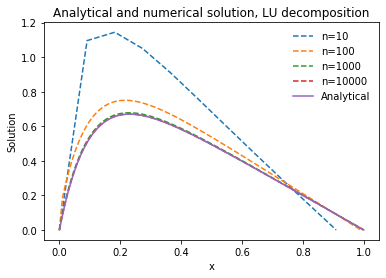
\includegraphics[width=0.8\columnwidth]{LU.png}
\caption{For n = 100 and higher we seem to get very similar results compared to the other two algorithms. For n = 10 we get a better results using LU decomposition. }
\label{fig:LU}
\end{figure}

LU decomposition produce very similar results to our own algorithm, except for n = 10, the LU decomposition method give a better result here. We can not however run the code using LU decomposition for higher n values than $10^4$. 


\begin{table}[H]
    \caption{Relative error}
    \label{tab:error}
    \begin{tabular}{|l |l |l| ll}% <-- Alignments: 1st column left, 2nd middle and 3rd right, with vertical lines in between
    \hline
      \textbf{n} & {Specialised algorithm} & {LU decomposition} \\ 
      \hline
      $10^1$ & 0.344692 &  -0.095737\\
       $10^2$ & 0.038877 $(10^{-2})$&  0.056614\\
      $10^3$ & 0.003950 $(10^{-3})$&  0.015716\\
      $10^4$ & 0.000396 $(10^{-4})$& 0.002682\\
      $10^5$ & 0.000040 $(10^{-5})$&  - \\ 
      $10^6$ &  0.000004 $(10^{-6})$& - \\ 
      $10^7$ & 0.000001 $(10^{-7})$& - \\ 
      $10^8$ & -0.001140 & - \\
      \hline
    \end{tabular}
\end{table} 

In table \ref{tab:error} we have calculated the relative error between the numerical and analytical solution of our specialised algorithm (the one where we exploited the fact that our diagonal elements were identical) and the LU decomposition. The error decreased for larger n's for our specialised algorithm until we tried n= $10^8$, where it suddenly increased.  For the LU decomposition we couldn't get results for n larger than $10^4$. At n=$10^3$ and n=$10^4$ the error is smaller for our algorithm, but at n=10 the error is much smaller for the LU method. This is consistent with what we saw in figures \ref{fig:method1}, \ref{fig:method2} and \ref{fig:LU}, where for n=10, results were better with LU decomposition. \\

We were also interested in knowing what the execution time was for the different algorithms, they can be found in table \ref{tab:time}. We have taken the average of running the code 5 times. We see here that the running time is very short with Lu decomposition for n = 10, n=$10^2$,  and n=$10^3$,  where the specialised algorithm is 10 times slower. However, at n=$10^4$, LU decomposition runtime jumps to around 17 seconds, whereas our algorithm stays the same. We can't run our LU method for n any higher than this, but for our own algorithm we see that the runtime increases by 10 from n=$10^5, 10^6,10^7,10^8$. 

\begin{table}[H]
    \caption{Execution time [seconds] (rounded off)}
    \label{tab:time}
    \begin{tabular}{|l |l |l| lll}% <-- Alignments: 1st column left, 2nd middle and 3rd right, with vertical lines in between
    \hline
      \textbf{n}& {Specialised algorithm} & {LU decomposition} \\ 
      \hline
      $10^1$ &  0.19885 & 0.02368\\
       $10^2$ & 0.19894 &  0.03877\\
      $10^3$ & 0.20114&  0.09070\\
      $10^4$ &0.32697 & 16.767 \\
      $10^5$ & 1.15458&   -\\ 
      $10^6$ & 9.19765&  -\\ 
      $10^7$ &  102.221& - \\ 
      $10^8$ & 1043.68 &  -\\
      \hline
    \end{tabular}
\end{table} 

\section{Discussion}

Our three algorithms produce the same results. The LU decomposition method can be used on any matrix, while our general and specialised case can only be used on tridiagonal matrices. Because of this we only need to iterate over three arrays, instead of a whole matrix. That's why our algorithm is so much faster than the LU decomposition (look at table \ref{tab:time}). When n is $10^5$ or higher, our LU program won't return any results. We can also see that there is a drastic increase in runtime at n = $10^4$. For n=$10^5$ we would need $10^{15}$ FLOPs, which would need an enourmous amount of memory. As the three algorithms gave the same results, if we have a tridiagonal matrix, it would be more efficient to use our own algorithm over the LU decomposition method, at least if our n is large.  \\

For the relative error there was a pattern for the specialised algorithm, where the relative error follows the truncation error $n^2$. As n increases, the relative error decreases. We expected it to increase again at around $10^7$, but with us it increased at $10^8$. I'm not sure what the minus sign means, but it does look like we have reached some limit where we are getting a loss of precision, because the step size, h, becomes too small. This leads to a round-off error and because of all the iterations we do, it can have a big impact on the resulting value. \\

The relative error also gave us a much larger value at n = 10 for our own algorithm, which indicates it may not hold up at small n. It may also be something in our code that is not right. For smaller n, up to $10^3$, it may be wise to use LU decomposition method, as it actually was faster at these values of n, and gave a better result at n = 10. But for larger matrices, our own algorithm performs better (given that we have a tridiagonal matrix). However, we should also take into account how much memory the LU method needs compared to our algorithm. If we have a matrix of dimensions 10 000 x 10 000, this will take up a lot of memory on our computer, and as most of us use laptops that may only have 8 GB of RAM, there is a chance of running out of memory. That is what happened to us in our program, when we got no results in our LU method for n larger than $n=10^4$.  \\


\section{Conclusion}

We see from this project the importance of having a thorough understanding of our problem and how our algorithms work, and to plan well before starting to actually code. Because we had a triangular matrix, we could make a simpler program that computed the problem faster, with less memory needed, instead of using the more common LU decomposition method. The three algorithms may approximately give the same results for a certain n, but we've seen that by tailoring our code for our problem, we reduced runtime and memory usage. 

\section{Github reference}

For all python codes and other material used for this project go to: 

https://github.com/beateovl/FYS-3150-4150.git



\bibliography{biblio.bib}{}
\bibliographystyle{apacite}


\end{document}